% create the chapter theoretical background
\chapter{Theoretical Background}

% section about antibiotic resistance
\section{Antibiotic resistance}

Antibiotic resistance is definied as the the ability of bacteria, viruses, fungi and parasites resists the antimicrobial medicines like for example antibiotics \cite{who_antibiotic_resistance}. Most commonly used antibiotics are the so called $\beta$-lactam antibiotics which contain a $\beta$-lactam ring in their chemical structure \cite{bush2013}. This includes penicillin, cephalosporin and carbapenems, which are the most common antibiotics used today \cite{versporten2018}. The enzymes in both Gram-positive and Gram-negative bacteria which are responsible for the resistance are called $\beta$-lactamases. Through hydrolysis, the enzymes break the $\beta$-lactam ring, which is the key structure of the $\beta$-lactam antibiotics \cite{ambler1980}. The core structure of the $\beta$-lactam antibiotics is shown in Figure \ref{fig:beta_lactam_antibiotics}.

\begin{figure}[htbp]
    \centering
    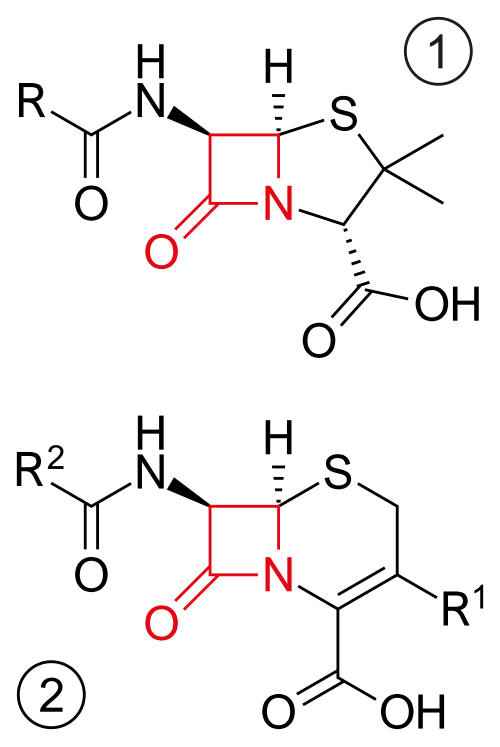
\includegraphics[width=0.6\textwidth]{resources/images/beta_lactam_antibiotics_example.png}
    \caption{Core structure of $\beta$-lactam antibiotics. The four-membered $\beta$-lactam ring is the key structural element responsible for the antibiotic activity (marked in red). The strucure shown in number one is the core of penicillins and the second one is the core of cephalosporins. \textbf{Source:} Wikipedia $\beta$-lactam antibiotics article \cite{wikipedia_beta_lactam_antibiotics}}
    \label{fig:beta_lactam_antibiotics}
\end{figure}

The $\beta$-lactam antibiotics exert their bactericidal effect by targeting the bacterial cell wall. They mimic the the D-Ala-D-Ala moiety of the peptidoglycan layer of the cell wall, which is the main component of the cell wall in bacteria. The active site residue prevents cross-linking of the peptidoglycan strands, compromising the cell wall integrity. The weakend cell is not longer able to withstand the osmotic pressure, leading to the cell lysis and death \cite{kim2023}.


% section about machine learning
\section{Machine learning}

